\chapter{Lattice study of a gauge-fermion-scalar theory}

The Standard Model electroweak theory is very successful in describing experimental results. However, some theoretical concerns suggest that a more consistent theory should be found. Specifically, the search for an alternative mechanism for the generation of masses is an active research field.
Composite Higgs models belong to this branch of Beyond the Standard Model (BSM) research.

In this chapter we discuss the lattice study of an SU(2) gauge theory coupled to fermions and scalars. This theory is intended as a minimal scenario for composite Higgs models, in which the problem of the generation of fermion masses is addressed via the fundamental partial compositeness mechanism \cite{Sannino:2016sfx}. 

The chapter is organised as follows. We start by exposing some of the reasons why the Standard Model Higgs mechanism turns out to be theoretically unappealing. Then we introduce composite Higgs models, and we explain what makes the generation of fermion masses a bit problematic in this setup. We then describe the mechanism of fundamental partial compositeness.
After setting these theoretical motivations, we move to the description of the specific theory under analysis, starting with some continuum aspects and then moving to the lattice setup. Finally,  we present the results obtained on the spectrum and phase space of the lattice theory.


%%%%%%%%%%%%%%%%%%%%%%%%%%%%%%%%%%%%%%%%%%%%%%%%%%

\section{Composite Higgs models and fundamental partial compositeness}


\subsection{The naturalness and triviality problems}

The Standard Model Higgs boson is an elementary scalar field. There exist some theoretical problems related to elementary scalars, known as naturalness and triviality problem. 

The naturalness problem is due to the fact that the Higgs mass is extremely sensitive to corrections arising from new physics, which may appear at a very high energy scale. We know the Standard Model to be an effective field theory, valid up to some ultraviolet cutoff $\Lambda_{SM}$, whose UV-completion is yet unknown. $\Lambda_{SM}$ will be at most equal to the Planck scale $M_{PL} = 10^{19} \: \mathrm{GeV}$, where a complete quantum theory of gravity should appear. 
When we consider the Standard Model (SM) as an effective theory, we do not restrict ourselves to the renormalisable operators of the SM Lagrangian, but we consider an effective Lagrangian containing all possible operators built with the SM elementary fields, which respect the symmetries of the SM:

\begin{equation}
\Lag_{eff} = \sum_{d=1}^{\infty} \frac{c_{(d)}}{\Lambda_{SM}^{d-4}} O^{(d)} \: ,
\end{equation}
%
where $d$ is the energy dimension of the operator $O^{(d)}$. For dimensional reasons, the coefficients of $d > 4$ operators are suppressed by a factor $\Lambda_{SM}^{- \abs{d-4}}$, while the coefficients of $d < 4$ operators are enhanced by a factor $\Lambda_{SM}^{\abs{d-4}}$. If we knew the UV-completion of the SM, i.e. a theory valid up to arbitrarily high energy scales, of which the SM is a low-energy effective description, then we could in principle compute the coefficients $c_{(d)}$ as functions of the parameters of the UV-complete theory.
 The quadratic term in the Higgs potential is the only $d<4$ operator present in $\Lag_{eff}$, specifically it is a $d=2$ operator. The tree-level Higgs mass is proportional to the coefficient of this operator. The fact that the Higgs is "light", together with the fact that new physics may come at a very high energy scale, contributes to creating a theoretically problematic scenario. If new physics appeared at a scale which is significantly larger than the TeV, then reconstructing the experimental value of 125 GeV for the Higgs mass would require the coefficient $c_{(2)}$ to be extremely small. As a consequence, the UV-completion accounting for the new physics would be constrained by the fact that $c_{(2)}$ must assume the required very small value. This scenario, in which the low-energy parameters of the theory constrain to a very high degree the UV-completion, defined at a much higher scale, is considered to be unnatural.
 
Elementary scalars may also be affected by the triviality problem \cite{Callaway:1988ya}. This problem is related to the running of the scalar quartic self-coupling. In a pure scalar field theory, defined by the Lagrangian
 
 \begin{equation}
 \Lag [\phi] = \frac{1}{2} \partial_{\mu} \phi \: \partial^{\mu} \phi - \frac{1}{2} m^2 \phi^2 - \frac{\lambda}{4!} \phi^4 \: ,
 \end{equation}
 %
 the renormalised quartic coupling at the momentum scale $p$, at lowest order in perturbation theory, is given by:
 
 \begin{equation}
 \bar \lambda (p) = \frac{\lambda_R}{1- \frac{3}{16 \pi^2}  \lambda_R \log\frac{p}{\mu}} \: ,
 \label{trivial_running}
 \end{equation}
 %
 where $\lambda_R$ is the renormalised coupling at the scale $p = \mu$. If $\lambda_R \neq 0$, there exists a finite momentum scale at which the renormalised coupling diverges, thus making the theory inconsistent. It seems that the only consistent theory is the noninteracting one, characterised by $\lambda_R = 0$. Should this be the case also for the SM Higgs field, the Higgs mechanism would be invalidated, since it is strongly based on the existence of the scalar self-interactions. 
 This argument however does not directly apply to the SM Higgs scalar, since gauge and Yukawa interactions must be also taken into account in order to compute the running of $\lambda$. The quartic coupling of the SM Higgs actually becomes negative at high energies, thus leading to problems related to the stability of the SM vacuum \cite{Degrassi:2012ry}. A scalar field theory is trivial whenever an ultraviolet fixed point for the quartic coupling is absent. In this case, the theory is ill-defined at high energies, unless the renormalised coupling is set to zero, thus eliminating scalar self-interactions. This supports the interpretation of the SM as an effective field theory, defined up to an ultraviolet cutoff, and discourages the introduction of elementary scalars in a UV-complete theory.
 


\subsection{Composite Higgs models}

Composite Higgs models constitute an alternative to the Higgs mechanism for the generation of masses, in which no elementary scalars are included. The first inspiration for composite Higgs models came from the fact that the Higgs vacuum expectation value is not the only source of electroweak symmetry breaking in the Standard Model. In fact, QCD pions contribute to the mass of the $W$ and $Z$ gauge bosons. This is due to the fact that electroweak symmetry is embedded in the chiral SU(2)$_L\times$SU(2)$_R$ symmetry of QCD, which is spontaneously broken by the strong dynamics.

It is shown in \cite{Susskind:1978ms} that, in a theory with the SM gauge symmetry SU(2)$_L\times$U(1)$_Y\times$SU(3)$_C$, containing one family of massless quarks and no Higgs doublet, the electroweak gauge bosons become massive.
Specifically, the $W^{\pm}$ bosons acquire a mass $M_{W} = (g/2) f_{\pi} \simeq 30 \: \mathrm{MeV}$, where $g$ is the \suEW gauge coupling, and $f_{\pi}$ the pion decay constant. Moreover, the photon is massless and the ratio of the $W$ and $Z$ masses is the same as in the SM. In order to obtain these results, the gauge couplings are assumed to run in the same way as in the SM. In particular, the SU(3)$_C$ gauge coupling becomes $\sim 1$ at 1 GeV, and the electroweak sector is treated as a small perturbation. The tree-level value of $g/2$ can be deduced from the relation between the Fermi constant $G_F$ and the $W$ boson mass:

\begin{equation}
\frac{G_F}{\sqrt 2} = \biggl( \frac{g}{2 \sqrt 2} \biggr)^2 \frac{1}{M_W^2}  \; ,
\end{equation} 
%
while the pion decay constant is given by $f_{\pi} = 93 \: \mathrm{MeV}$ \cite{Peskin:1995ev}.

The $W$ boson mass thus generated is clearly too small with respect to the experimental value of 80 GeV, and indeed in the SM the almost unique source of electroweak symmetry breaking is the Higgs vacuum expectation value. However, one may imagine a "scaled-up" version of QCD, where the pion decay constant is big enough to provide a realistic mass for $W$ and $Z$ bosons. This is the idea behind Technicolor (TC) models \cite{Weinberg:1975gm,Susskind:1978ms}. In these models, all the SM particles are included except for the Higgs doublet, and on top of that a new strongly interacting sector is added. The new sector contains fermionic matter, which we will refer to as TC-fermions, and a new non-Abelian gauge interaction. The TC sector in isolation is symmetric under a global flavour symmetry, which is assumed to be spontaneously broken by the formation of the TC-fermion condensate. The flavour symmetry is required to have an SU(2)$\times$U(1) subgroup, so as to allow the embedding of electroweak interactions. Specifically, the SU(2)$_L\times$U(1)$_Y$ generators are identified with some of the broken generators of the TC flavour symmetry. As a consequence, the $W$ and $Z$ bosons acquire a mass proportional to the TC-pion decay constant. In these models the Higgs boson is identified with the lightest scalar resonance of the TC-sector. In general it is not automatic to obtain both a Higgs mass and $W$ and $Z$ masses in good agreement with experimental values. In particular, unless some care is taken, the Higgs boson will end up being heavier than the measured 125 GeV. Walking Technicolor models \cite{Yamawaki:1985zg,Dietrich:2005jn,Appelquist:2010gy} address this kind of issue.

Another composite Higgs scenario is the one of composite Goldstone Higgs models \cite{Kaplan:1983sm,Kaplan:1983fs}. In these models a new strongly interacting sector analogous to the TC one is introduced (we will continue to call it TC sector), but the embedding of electroweak symmetry is substantially different. In fact, the SU(2)$_L\times$U(1)$_Y$ generators are identified with some of the unbroken generators of the TC flavour symmetry, so that $W$ and $Z$ bosons remain massless. The Higgs is identified with one of the Goldstone bosons of the broken flavour symmetry. Unless some explicit breaking of this symmetry is introduced, the Goldstone-Higgs is a massless particle. In order to generate the correct Higgs mass and to give masses to $W$ and $Z$, some new interactions are introduced, which explicitly break the TC flavour symmetry. The explicit form of possible symmetry-breaking interactions will be discussed in the next section, in the case of a specific model. In the setup of composite Goldstone Higgs models, the Higgs boson is naturally light and a large separation occurs between the electroweak scale and the scale at which the TC gauge coupling becomes strong. Therefore the masses of non-Goldstone TC-hadrons are expected to be large with respect to the electroweak scale, and possibly beyond the range explored so far in accelerator experiments.

To conclude, we remark that in composite Higgs models electroweak symmetry is broken as a consequence of the dynamics of the theory. In this respect, these models are more theoretically satisfactory than the SM, where electroweak symmetry breaking is simply modelled and no dynamical reason is given for its occurrence. In the next section we analyse in some more detail the SU(2) gauge theory with two fermions in the fundamental representation, which can serve as setup for both Technicolor and composite Goldstone Higgs scenarios \cite{Cacciapaglia:2014uja}.


\subsection{SU(2) + 2 fermions as minimal composite Higgs model}
\label{SU2_composite_Higgs}

In this section, following the lines of \cite{Cacciapaglia:2014uja}, we discuss a specific model: the SU(2) gauge theory with two fermions in the fundamental representation. This is a good candidate for being the TC sector in both a Technicolor and a composite Goldstone Higgs scenario.

The Lagrangian of this model is given by:

\begin{equation}
\Lag = - \frac{1}{4} F_{\mu\nu}^a F^{a\mu\nu}  + \bar u (i \slashed D - m) u + \bar d (i \slashed D - m) d \: ,
\label{SU2_Lagrangian}
\end{equation}
%
where $u$ and $d$ are the two TC-fermion fields with equal mass $m$, $F_{\mu\nu}^a$ is the non-Abelian field strength tensor and $D_{\mu}$ is the covariant derivative. In the case $m=0$, this Lagrangian has a larger flavour symmetry than the SU(2)$_L \times$SU(2)$_R$ generally expected for an SU(N) gauge theory with two fundamental fermions. This is due to the fact that the fundamental representation of SU(2) is pseudo-real, i.e. there is a relation between a matrix of SU(2) and its complex conjugate:

\begin{equation}
U = (-i \sigma^2) U^* (i \sigma^2) \: , \quad U \in\mathrm{ SU}(2) \: ,
\label{pseudoreal}
\end{equation}
%
where $\sigma^2$ is the second Pauli matrix.
Due to this property, we can define an enlarged flavour multiplet of left-handed fields transforming under the fundamental representation of SU(2):

\begin{equation}
Q = 
\begin{pmatrix}
u_L \\
d_L \\
\tilde u_L \\
\tilde d_L
\end{pmatrix} \: , 
\end{equation}
%
where the left- and right-handed spinors are defined by: 

\begin{equation}
u_L = \frac{\id - \gamma_5}{2}u \: ,  \quad u_R = \frac{\id + \gamma_5}{2}u \: , \quad  d_L = \frac{\id - \gamma_5}{2}d \: ,  \quad d_R = \frac{\id + \gamma_5}{2}d \: ,
\end{equation}
%
and we have defined some new left-handed fields $\tilde u_L$ and $\tilde d_L$ as:

\begin{equation}
\tilde u_L = -i \sigma^2 C \bar u_R^T \: , \quad \tilde d_L = -i \sigma^2 C \bar d_R^T \: .
\label{ud_tilde}
\end{equation}
%
In equation \ref{ud_tilde}, the matrix $-i \sigma^2$ acts on the colour indices of the spinors, while $C$ is the charge conjugation operator, acting on Dirac indices (see appendix \ref{gamma_matrices}). As a consequence of equation \ref{pseudoreal}, $\tilde u_L$ and $\tilde d_L$ transform under the fundamental representation of the TC group SU(2):

\begin{center}
\begin{tikzcd}
u_R \to u'_R = Uu_R, \quad U \in \mathrm{SU}(2)   \arrow[d,Rightarrow] \\ 
 \tilde u'_L = -i \sigma^2 C  \bar {u'}_R^T = -i \sigma^2  U^* C  \bar u_R^T =  U  \tilde u_L \: .
\end{tikzcd}
\end{center}

The Lagrangian \ref{SU2_Lagrangian}  can be rewritten in terms of $Q$ as follows:

\begin{equation}
\Lag = - \frac{1}{4} F_{\mu\nu}^a F^{a\mu\nu}  + i \bar Q \slashed D Q  + \frac{m}{2} Q^T (-i \sigma^2) C E Q +  \frac{m}{2} (Q^T (-i \sigma^2) C E Q)^{\dagger} \: ,
\label{SU2_Lagrangian2}
\end{equation}
%
where

\begin{equation}
E =
\begin{pmatrix}
0 & 0 & 1 & 0 \\
0 & 0 & 0 & 1 \\
-1 & 0 & 0 & 0 \\
 0 & -1 & 0 & 0
\end{pmatrix} \: .
\end{equation}
%
If $m=0$, this Lagrangian is symmetric under global SU(4) transformations of the multiplet $Q$, while if $m \neq 0$ the symmetry is reduced to the subgroup Sp(4), defined as being the group of transformations such that the following condition is verified:

\begin{equation}
E T_n + T_n^T E = 0\: ,
\end{equation}
%
where $T_n$ are the fifteen generators of the fundamental representation of SU(4).

After defining the  TC sector in isolation, we  embed electroweak symmetry by assigning the following transformation properties:

\begin{itemize}
\item $Q_L = (u_L,d_L)^T$ is an SU(2)$_L$ doublet with zero hypercharge
\item $\tilde u_L$  and $\tilde d_L$ are two SU(2)$_L$ singlets with hypercharges -1/2 and +1/2 respectively. 
\end{itemize}
%
With these assignments, we can identify the electroweak generators among the generators of flavour symmetry. First of all, we list the generators of SU(4), and, for future purposes, we split them into two groups, denoted by $S^i$, $i = 1, \dots , 10$, and $X^j$, $j = 1, \dots, 5$:


 \begin{equation}
\begin{split}
& S^ {1,2,3} = \frac{1}{2}
\begin{pmatrix}
\sigma^i & 0 \\
0 & 0
\end{pmatrix} \: , \quad
S^ {4,5,6} = \frac{1}{2}
\begin{pmatrix}
0 & 0 \\
0 & -\sigma^{iT}
\end{pmatrix} \: ,  \quad \\
S^ {7,8,9} & = \frac{1}{2 \sqrt 2}
\begin{pmatrix}
0 & i \sigma^i \\
-i \sigma^i & 0
\end{pmatrix} \: , \quad
S^{10} = \frac{1}{2 \sqrt 2}
\begin{pmatrix}
0 & 1 \\
1 & 0
\end{pmatrix} \: , 
\end{split} 
\label{S}
\end{equation}

 \begin{equation}
\begin{split}
X^1 = \frac{1}{2 \sqrt 2}
& \begin{pmatrix}
0 & \sigma^3 \\
\sigma^3 & 0
\end{pmatrix} \:  , \quad
X^2 = \frac{1}{2 \sqrt 2}
\begin{pmatrix}
0 & -i \\
-i & 0
\end{pmatrix} \: ,  \quad 
X^3 = \frac{1}{2 \sqrt 2}
\begin{pmatrix}
0 & \sigma^1 \\
\sigma^1 & 0
\end{pmatrix} \: ,  \quad \\
& X^4 = \frac{1}{2 \sqrt 2}
\begin{pmatrix}
0 & \sigma^2 \\
\sigma^2 & 0
\end{pmatrix} \: , \quad
X^5 = \frac{1}{2 \sqrt 2} 
\begin{pmatrix}
1 & 0 \\
0 & -1
\end{pmatrix} \: ,
\end{split} 
\label{X}
\end{equation}
%
where, as usual, $\sigma^i$,  $i = 1,2,3$, are the Pauli matrices. Due to the transformation properties of $Q_L$, $\tilde u_L$ and $\tilde d_L$ under the electroweak gauge group, $S^{1,2,3}$ are identified with the generators of SU(2)$_L$, while $S^6$ is the generator of U(1)$_Y$.

We now assume that the TC sector in isolation, in the SU(4)-symmetric case $m=0$, undergoes spontaneous flavour symmetry breaking due to the formation of the TC-fermion condensate:

\begin{equation}
\langle Q^T(-i \sigma^2) C \Sigma_0 Q + (Q^T(-i \sigma^2) C \Sigma_0 Q)^{\dagger} \rangle \neq 0 \: .
\end{equation}
%
The SU(4) flavour symmetry is broken down to the subgroup spanned by the  unbroken generators, which fulfil the following condition:

\begin{equation}
 \Sigma_0 T_n + T_n^T \Sigma_0  = 0 \: .
\end{equation}
%
$\Sigma_0$ is a yet unspecified matrix in flavour space, whose alignment with respect to the electroweak generators will be determined by minimising the effective potential of the theory in interaction with the electroweak group, taking into account also possible symmetry-breaking perturbations. 

 We rewrite $\Sigma_0$ as  the superposition:

\begin{equation}
\Sigma_0 = \cos \theta \:  \Sigma_B + \sin \theta \: \Sigma_H \: ,
\end{equation}
%
where 

\begin{equation}
\Sigma_B =
\begin{pmatrix}
i \sigma^2 & 0 \\
0 & -i \sigma^2
\end{pmatrix} \:  , \quad
\Sigma_H = E =
\begin{pmatrix}
0 & \id \\
-\id &  0 
\end{pmatrix} \: . 
\end{equation}
%
If $\Sigma_0 = \Sigma_B$, the unbroken generators are the $S^i$'s defined in equation \ref{S}, while the broken generators are the $ X ^j$'s of equation \ref{X}. In particular,  electroweak symmetry is preserved.  If $\Sigma_0 = \Sigma_H$, the unbroken generators are:

\begin{equation}
S^1 + S^4 \: , \quad S^2 + S^5 \: , \quad S^3 + S^6 \: , \quad S^{7,9,10} \: , \quad X^{1, 2 ,3, 5} \: ,
\end{equation}
%
and the broken ones:

\begin{equation}
S^1 - S^4 \: , \quad S^2 - S^5 \: , \quad S^3 - S^6 \: , \quad S^8 \: , \quad  X^4  \: .
\end{equation}
%
In this case electroweak symmetry is broken. Moreover, we will see in  the following that, for $\theta = \pi/2$, the mass of the $W^{\pm}$ bosons is directly determined by the Goldstone-boson decay constant and the SU(2)$_L$ coupling constant, as in Technicolor models. It follows that a model with $\theta = \pi/2$ is a good candidate for Technicolor, while a model with $\theta \sim 0$ could work as composite Goldstone Higgs scenario.

For a generic alignment $\theta$, the broken generators are given by the following combinations: 

\begin{equation}
\begin{split}
Y^1 = c_{\theta} X^1 - s_{\theta} \frac{S^1-S^4}{\sqrt  2} \: , & \quad Y^2 = c_{\theta} X^2 + s_{\theta} \frac{S^2-S^5}{\sqrt  2} \: , \quad Y^3 = c_{\theta} X^3 + s_{\theta} \frac{S^3-S^6}{\sqrt  2} \: , \quad \\
& Y^4 = X^4 \: ,  \quad  Y^5 = c _{\theta} X^5 - s_{\theta} S^8  \: ,
\end{split}
\end{equation}
%
where $c _{\theta} = \cos \theta$ and $s _{\theta} = \sin \theta$. 
In order to study the phenomenology of the low-energy excitations of this model, the effective Lagrangian approach can be used. We define the Goldstone matrix as:

\begin{equation}
\Sigma = e^{i \frac{\phi^a}{f} Y^a} \Sigma_0 \: ,
\end{equation}
%
where $\phi^a(x)$, $a = 1, \dots , 5$, are the Goldstone boson fields and $f$ the Goldstone boson decay constant.
The kinetic term of the effective Lagrangian, where the electroweak interactions are introduced via the covariant derivative $D_{\mu}$, is given by:

\begin{equation}
f^2 \tr [(D_{\mu} \Sigma)^{\dagger} D^{\mu} \Sigma ] \: ,
\label{eff_lagrangian}
\end{equation}
%
where

\begin{equation}
D_{\mu} \Sigma = \partial_{\mu} \Sigma -i (G_{\mu}^T \Sigma + \Sigma G_{\mu}) \: ,
\end{equation}

\begin{equation}
G_{\mu} = g W^i_{\mu} S^i + g' B_{\mu} S^6 \: , \quad i = 1,2,3 \: .
\end{equation}
%
In the previous equation, $g$ is the SU(2)$_L$ coupling, $g'$ the U(1)$_Y$ coupling and $W^i_{\mu}$, $B_{\mu}$ their respective gauge boson fields.

In \cite{Cacciapaglia:2014uja}, computations are carried on in the unitary gauge, i.e. by fixing to zero the Goldstone boson fields which provide the longitudinal degrees of freedom of $W$ and $Z$. In our case this means: $\phi^{1,2,3} = 0$. The remaining Goldstone bosons are renamed as: $\phi^4 \equiv h$, $\phi^5 \equiv \eta$. The Goldstone matrix in the unitary gauge reads:

\begin{equation}
\Sigma = e^{\frac{i}{f} (h Y^4 + \eta Y^5)} \Sigma_0 \: .
\label{Gold_matrix_ug}
\end{equation}
%
By inserting \ref{Gold_matrix_ug} in \ref{eff_lagrangian}, and expanding in powers of $\eta/f$, $h/f$, one finds the masses and couplings of the fields $W^{\pm}$, $Z$, $h$ and $\eta$. $W^i$ and $B$ are expressed in terms of $W^{\pm}$, $A$ and $Z$ as in equations (\emph{must be added in the introduction}). The resulting gauge boson masses are:

\begin{equation}
m^2_{W} = 2 g^2 f^2 s_{\theta}^2 \: ,
\end{equation}

\begin{equation}
m^2_Z = 2 (g^2 + {g'}^2) f^2 s_{\theta}^2 = \frac{m_W^2}{\cos^2\theta_W} \: ,
\end{equation}
%
where $\theta_W$ is the Weinberg angle. The Goldstone bosons $h$ and $\eta$ are massless (at tree level), and their couplings to the electroweak gauge bosons are given by:

\begin{equation}
g_{hWW} = \sqrt 2 g^2 f s_{\theta} c_{\theta} = g m_W c_{\theta} = g^{SM}_{hWW} c_{\theta} \: ,
\end{equation}

\begin{equation}
g_{hZZ} = \sqrt 2 (g^2 + {g'}^2) f s_{\theta} c_{\theta} = \sqrt{g^2 + {g'}^2} m_Z c_{\theta} = g^{SM}_{hZZ} c_{\theta} \: ,
\end{equation}

\begin{equation}
g_{hhWW} = \frac{1}{4} g^2 c_{2 \theta} = g_{hhWW}^{SM} c_{2 \theta} \; ,
\end{equation}

\begin{equation}
g_{hhZZ} = \frac{g_{hhWW}}{2 \cos^2 \theta_W}  = g_{hhZZ}^{SM} c_{2 \theta} \; ,
\end{equation}

\begin{equation}
g_{\eta \eta WW} = - \frac{1}{4} g^2 s_{\theta}^2 \; ,
\end{equation} 

\begin{equation}
g_{\eta \eta ZZ} = \frac{g_{\eta \eta WW}}{2 \cos^2 \theta_W}  \; .
\end{equation}
%
It can be seen that for $\theta \sim 0$ the couplings of  $h$ to $W$ and $Z$ are very similar to the ones of the Standard Model Higgs, while the couplings of $\eta$ are suppressed by a factor $s_{\theta}^2$. Moreover, if $\theta \sim 0$, the scale hierarchy $f \gg m_W$ is realised,  according to which the TC-hadron masses are expected to be much larger than the electroweak scale. This is the limit in which the composite Goldstone Higgs scenario is realised. If $\theta$ is significantly larger than zero, the $h$ particle stops looking similar to the Higgs, and the Higgs role is assumed by the lightest scalar resonance of the TC sector, as in Technicolor. If $\theta = \pi/2$, the two scalar particles $h$ and $\eta$ become degenerate (their couplings to $W$ and $Z$ are equal), and the associated complex state is stable and can play a role as dark matter candidate \cite{Cacciapaglia:2014uja}.

Unless flavour symmetry is explicitly broken, all the possible alignments of $\Sigma_0$ are equivalent. The introduction of electroweak interactions via partial gauging of SU(4) results in the explicit breaking of flavour symmetry. Gauge boson loops induce a potential for the Goldstone bosons, which is minimised by a specific value of the alignment angle $\theta$. Moreover, also other possible symmetry-breaking contributions, such as interactions with SM fermions and mass terms for the TC-fermions, contribute to the potential, and influence the alignment of $\Sigma_0$. It is shown in \cite{Cacciapaglia:2014uja} that the contribution of gauge boson loops to the one-loop potential contains mass terms for $h$ and $\eta$, and is minimised at $\theta = 0$, corresponding to preserved electroweak symmetry.


A complete model of composite Higgs will contain some extra interactions on top of the ones mentioned until now, which are meant to generate masses for the SM fermions. For example, concentrating on the top quark mass, one could add to the Lagrangian \ref{SU2_Lagrangian2} an effective four-fermion operator of the form:

\begin{equation}
\frac{y_t}{\Lambda_t^2} \bar q_L t_R \bar u_R  Q_L  + \mathrm{h.c.} \: ,
\label{}
\end{equation}
%
where $q_L$ is the left-handed doublet containing the SM top and bottom quarks, $q_L = (t_L  \: b_L)^T$, and $t_R$ is the right-handed top quark. $u_R$ and $Q_L = (u_L \: d_L)^T$ are TC-fermion fields. This is just an effective operator, which indicates that the theory should be extended by including some new interactions at energies larger than $\Lambda_t$. The contribution of this operator to the one-loop potential is minimised at $\theta = \pi/2$, i.e the Technicolor-like alignment \cite{Cacciapaglia:2014uja}.

The last source for the Goldstone boson potential analysed in \cite{Cacciapaglia:2014uja} is a mass term for the TC-fermions. This term is assumed to be symmetric under SU(2)$_L \times$U(1)$_Y$, and therefore proportional to $\Sigma_B$: $M = \mu \Sigma_B$. It is found that, at the price of some fine tuning between the contributions of the top loop and the TC-fermion mass term, a small value of $\theta$ can be obtained, thus realising the composite Goldstone Higgs scenario.

The construction made until now is based on the assumption that the spontaneous symmetry breaking pattern SU(4)~$\to$~Sp(4)  is realised in the TC sector in isolation. This assumption must be verified via lattice simulations. Lattice studies of the SU(2) gauge theory with two fundamental fermions have found clear signs of symmetry breaking \cite{Arthur:2016dir}: Goldstone boson states have been observed whose mass vanishes in the limit of vanishing fermion mass while the associated decay constant remains finite. Moreover, lattice simulations are the only way for measuring the mass spectrum of the theory, indicating in which energy range new particles are to be expected. In the case of the SU(2) model with two fundamental fermions, the lightest resonances have been found to lie beyond the present LHC limits, even in the Technicolor limit $\theta = \pi/2$ \cite{Arthur:2016dir}.


\subsection{Fermion masses and partial compositeness}

The setup of composite Higgs models must be extended in order to include massive fermion states. This is usually done by introducing in the Lagrangian operators which couple the SM fermions to the TC-fermions. The couplings can involve SM fermion bilinears, as in extended Technicolor \cite{Dimopoulos:1979es,Eichten:1979ah}:

\begin{equation}
\frac{\lambda_t}{\Lambda_{UV}^{d-1}} \bar q_L \mathcal O t_R + \mathrm{h.c.} \: ,
\label{ETC}
\end{equation}
%
or can be linear in the SM fermions, as in partial compositeness \cite{Kaplan:1991dc}:

\begin{equation}
\frac{\lambda_t}{\Lambda_{UV}^{d_L - 5/2}} \bar q_L \mathcal O^L + \frac{\bar \lambda_t}{\Lambda_{UV}^{d_R - 5/2}} \bar t_R  \mathcal O^R + \mathrm{h.c.} \: .
\label{partial_compositeness}
\end{equation}
%
In the previous equations we only listed the operators participating in the generation of the top quark mass. $q_L = (t_L \: b_L)$ represents the SM third quark family left-handed doublet, $t_R$ the right-handed top quark and $\mathcal O$, $\mathcal O^L$, $\mathcal O^R$ composite operators of the TC sector. Generally the operators of equations \ref{ETC}, \ref{partial_compositeness} are non-renormalisable, and the theory must be extended with new interactions at energies larger than $\Lambda_{UV}$. The operators \ref{ETC}, \ref{partial_compositeness} thus arise as low-energy effective operators, accompanied by a power of $\Lambda_{UV}$ dictated by the scaling dimension of $\mathcal O$, $\mathcal O^L$, $\mathcal O^R$ ($d$, $d_L$, $d_R$). The particle content of the TC sector must be chosen in such a way that the composite operators can have the correct quantum numbers for coupling with SM fermions. In particular the operator $\mathcal O$ of equation \ref{ETC} must have the same quantum numbers as the SM Higgs, while $\mathcal O^L$ and $\mathcal O^R$ of equation \ref{partial_compositeness} must have spin $1/2$ and, on top of the electroweak quantum numbers, must also carry SU(3)$_C$ charge. This means that, in the partial compositeness setup, the SU(3)$_C$ symmetry must be embedded in the TC-fermion flavour symmetry, in such a way that it is not broken by the TC-fermion condensate.

In the partial compositeness scenario, fermion masses are generated via mixing between SM fermions and fermionic composite states of the TC sector. We denote by $\Lambda_{TC} < \Lambda_{UV} $ the scale at which the TC gauge coupling becomes strong, and we consider the effective theory arising when the ultraviolet cutoff is fixed to $\Lambda_{TC}$. In the model considered in \cite{Kaplan:1991dc}, the operators $\mathcal O^L$, $\mathcal O^R$ mediate the coupling of the top quark to the same fermionic resonance $B$. The interactions in the effective Lagrangian look like:

\begin{equation}
\Lag_{eff}^{int} = c \Lambda_{TC}  \bigl( \lambda_t(\Lambda_{TC}) \bar t_L B_R + \bar \lambda_t(\Lambda_{TC}) \bar t_R B_L \bigr) - m_B \bar B_L B_R + \mathrm{h.c.} \; ,
\end{equation}
%
where $c$ is an unknown coefficient and $\lambda_t(\Lambda_{TC})$, $\bar \lambda_t(\Lambda_{TC})$ are the coefficients appearing in equation \ref{partial_compositeness} evolved down to the scale $\Lambda_{TC}$. Under the assumption $(c \Lambda_ {TC})^2  \lambda_t(\Lambda_{TC}) \bar \lambda_t(\Lambda_{TC})/m_B^2 \ll 1$, the mass matrix has one light eigenvalue with mass

\begin{equation}
m_t \sim \frac{\lambda_t(\Lambda_{TC}) \bar \lambda_t(\Lambda_{TC})}{m_B} (c \Lambda_{TC})^2 \; ,
\end{equation}
%
and one heavier eigenvalue with mass $\sim m_B$. The physical top quark is identified with the light eigenstate, which is a superposition of the SM top and a TC composite state. This is the reason for the name partial compositeness: physical states are superpositions of elementary and composite states. The model proposed in \cite{Kaplan:1991dc}, when extended to three families of SM quarks and leptons, is able to generate a large hierarchy of masses among the three families, having the first and second families much lighter than the third, even though a very general flavour structure is assumed in the underlying microscopic theory.

In the context of partial compositeness, it is difficult to generate a realistic top quark mass, without at the same time introducing flavour changing neutral currents (FCNC) incompatible with experimental constraints. In fact, the microscopic interactions that generate the operators \ref{partial_compositeness}  in general generate also couplings among four SM fermions, which may lead to large FCNC. For this reason, it is desirable to have a large separation between the scale of the new microscopic interactions and the scale at which the TC interaction becomes strong ($\Lambda_{UV} \gg \Lambda_{TC}$), thus suppressing the contribution from unwanted FCNC. However, this constraint suppresses the value of the top mass as well. It is usually assumed that the TC sector is close to a fixed point at energies $\sim \Lambda_{UV}$, so that:

\begin{equation}
\frac{\lambda_t}{\Lambda_{UV}^{d_L - 5/2}}  = \frac{\lambda_t(\Lambda_{TC})}{\Lambda_{TC}^{d_L - 5/2}} \; , \quad \frac{\bar \lambda_t}{\Lambda_{UV}^{d_R - 5/2}}  = \frac{\bar \lambda_t(\Lambda_{TC})}{\Lambda_{TC}^{d_R - 5/2}} \: .
\end{equation}
%
It follows that the couplings relevant for the generation of the top quark mass are suppressed by a power of $\Lambda_{TC}/\Lambda_{UV}$:

\begin{equation}
\lambda_t (\Lambda_{TC}) =  \lambda_t \biggl( \frac{\Lambda_{TC}}{\Lambda_{UV}} \biggr)^{d_L - \frac{5}{2}} \; , \quad \bar \lambda_t (\Lambda_{TC}) =  \bar \lambda_t \biggl( \frac{\Lambda_{TC}}{\Lambda_{UV}} \biggr)^{d_R - \frac{5}{2}} \; .
\end{equation}
%
A large value of $\Lambda_{TC}/\Lambda_{UV}$ is needed to satisfy the constraints on FCNC, while a small value would be needed for predicting a realistic top mass.

One may still obtain results compatible with experiments if the scaling dimensions of $\mathcal O^L$ and $\mathcal O^R$ are such that $d_L , d_R \sim 5/2$. We consider for example a model in which the fermionic operators $\mathcal O^L$, $\mathcal O^R$ are given by the product of three TC-fermion fields. In this case:

\begin{equation}
d_L = \frac{9}{2} - \gamma_L \; , \quad d_R = \frac{9}{2} - \gamma_R   \; ,
\end{equation}
%
where $\gamma_{L,R}$ are the anomalous dimensions. Large anomalous dimensions $\gamma_{L,R} \sim 2$ would make it possible to have a large top mass, and at the same time suppressed FCNC. In fact, operators containing four SM fermions, responsible for FCNC, are not expected to develop large anomalous dimensions, since SM fermions are not coloured under the  TC gauge interaction \cite{Kaplan:1991dc}. 

Recent studies indicate that the required large anomalous dimensions are hard to achieve. In particular, in \cite{Pica:2016rmv} the SU(3) gauge theory with fundamental fermions is considered. The number of fermions is chosen in such a way that the theory is inside the conformal window, i.e. it has a nontrivial infrared fixed point. It is observed that the anomalous dimension of baryonic operators remains small down to the lowest point in the conformal window that can be analysed in perturbation theory. For a more detailed discussion of the conformal window see section \ref{ conformal_window}


\subsection{Fundamental Partial Compositeness}

In order to overcome the difficulties related to the generation of fermion masses in composite Higgs scenarios, models of fundamental partial compositeness have recently been introduced \cite{Sannino:2016sfx}. In these models, the TC sector contains as matter fields not only fermions but also scalars. The Lagrangian can be written schematically as follows:

\begin{equation}
\Lag = \Lag_{SM}^{H=0} + \Lag_{TC}^{kin} + \Lag_Y -V_S \; ,
\end{equation}
%
where $\Lag_{SM}^{H=0}$ is the SM Lagrangian without the  Higgs sector, $\Lag_{TC}^{kin}$ is the kinetic Lagrangian of the TC sector, containing eventual mass terms of TC-fermions and TC-scalars, $ \Lag_Y$ contains Yukawa interactions among SM fermions, TC-fermions and TC-scalars, and $V_S$ is the TC-scalar quartic potential.

The interactions between SM fermions and TC-fermions are mediated by Yukawa couplings with TC-scalars. At energies lower than $\Lambda_{TC}$,  interactions between SM fermions and composite fermionic states formed by one TC-fermion and one TC-scalar are thus generated, and  SM fermion masses arise via the partial compositeness mechanism. The name "fundamental" is due to the fact that only renormalisable operators appear in the Lagrangian.
The low-energy effective field theory arising from this setup has been studied in detail in \cite{Cacciapaglia:2017cdi}. The implications for flavour physics and the compatibility with precision measurements of a minimal realisation of this scenario, i.e. containing the minimal number of new elementary particles, have been analysed in \cite{Sannino:2017utc}. 

One may argue that, due to the presence of elementary scalars, models of fundamental partial compositeness are affected by the naturalness and triviality problems in the same way as the SM. While it is true that the naturalness problem is reintroduced, the scalars of fundamental partial compositeness may be free from the triviality problem. In fact, an ultraviolet fixed point may be present in the flow  of the scalar quartic couplings. We will discuss this point in more detail in section \ref{running_lambda}. Moreover, the constraint $d_{L,R} \sim 5/2$ on the scaling dimensions of the operators $\mathcal O^{L,R}$ of equation \ref{partial_compositeness} seems to indicate that operators with the scaling dimension of elementary scalars $d \sim 1$ must be present in the TC sector, which should mediate Yukawa-like couplings between SM fermions and TC-fermions. Therefore one may expect any purely fermionic realisation of partial compositeness to look at the effective level as the model described here \cite{Sannino:2016sfx} . Another interesting feature of the fundamental partial compositeness setup is that a complete theory of flavour is realised in a relatively self-contained way. This scenario offers a complete alternative to the Higgs mechanism of the SM.

As in the case of ordinary composite Higgs models, the pattern of global symmetry breaking assumed for the TC sector in isolation must be verified via lattice simulations. Specifically, in the model described in \cite{Cacciapaglia:2017cdi}, the symmetry breaking pattern in the fermion sector is assumed to be SU($2N_f$)$\to$Sp($2N_f$), where $N_f$ is the number of Dirac TC-fermion fields. The enlarged flavour symmetry SU($2N_f$) can be defined due to the fact that the gauge group is chosen as having a pseudo-real fundamental representation. In realistic models of fundamental partial compositeness, featuring more than one TC-scalar field, also the scalar sector is characterised by a global flavour symmetry. In the model described in \cite{Cacciapaglia:2017cdi}, the scalar flavour symmetry is assumed not to be spontaneously broken by the formation of a scalar condensate. This assumption should also be tested on the lattice. Lattice measurements of the Wilson coefficients determined by the strong dynamics would also be of great interest in the context of the low-energy effective  theory \cite{Cacciapaglia:2017cdi}. With these motivations, we started a lattice study of the SU(2) gauge theory with two fundamental fermions and one fundamental scalar. While this is not a realistic TC sector for a fundamental partial compositeness model, which would require multiple scalar fields, it is a good setup for a preliminary analysis of the impact of scalar fields on the symmetry breaking pattern and on the spectrum of composite states.


%%%%%%%%%%%%%%%%%%%%%%%%%%%%%%%%%%%%%%%%%%%%%%%%%%%%%%%

\section{Perturbative aspects of the continuum theory}
\label{running_lambda}

The object of our lattice analysis is the SU(2) theory with two fundamental fermions and one fundamental scalar. Before entering in the details of the lattice study, we mention some  interesting aspects of the continuum theory, related to the running of the scalar quartic couplings. 

For these first considerations, we analyse a more general model, with SU($N$) gauge group, and $N_f$ fermions and $N_S$ scalars in the fundamental representation.
We organise the scalar and fermion fields into matrices carrying a colour index $\alpha$ and a flavour index $i$: $S_{\alpha i}$, $Q_{\alpha i}$, and we write the Lagrangian as:

\begin{equation}
\Lag = -\frac{1}{4} F_{\mu\nu}^a F^{a \mu\nu} + \tr \bigl[ \bar Q i \slashed D Q\bigr] + \tr \bigl[ (D_{\mu}S)^{\dagger} D^{\mu} S\bigr] - V_S \: ,
\end{equation}
%
where $V_S$ is the scalar quartic potential. The most general quartic operators invariant under both SU($N$) and a global SU($N_S$) flavour symmetry are:

\begin{equation}
\bigl( \tr \bigl[ S^{\dagger} S \bigr] \bigr)^2 = S^*_{i \alpha} S_{\alpha i} S^*_{j \beta} S_{\beta j} \: , \quad 
\tr \bigl[ S^{\dagger} S S^{\dagger} S \bigr] = S^*_{i \alpha} S_{\alpha j} S^*_{j \beta} S_{\beta i} \: .
\label{quartic_operators}
\end{equation}
%
It follows that the scalar quartic potential, respecting colour and flavour symmetries, is given by:

\begin{equation}
V_S = \lambda_1 \bigl( \tr \bigl[ S^{\dagger} S \bigr] \bigr)^2 + \lambda_2 \tr \bigl[ S^{\dagger} S S^{\dagger} S \bigr]  \: .
\label{quartic_potential}
\end{equation}
%
If $N_S =1$, the two operators of equation \ref{quartic_operators} are equal, and one single scalar quartic coupling $\lambda = \lambda_1 + \lambda_2$ is present in the Lagrangian. Since it is of interest for the model studied in this thesis, we specialise the following considerations to the case $N_S = 1$. A complete analysis with generic $N_S$ has been carried out in \cite{Hansen:2017pwe}.

The one-loop beta functions of the gauge coupling $g$ and the scalar quartic coupling $\lambda$ are given by:

\begin{equation}
\begin{split}
 & (4 \pi)^2 \beta_g = - \biggl( \frac{11}{3} N - \frac{2}{3} N_f - \frac{1}{6} \biggr) g^3 \: ,\\
 & (4 \pi)^2 \beta_{\lambda} = 4(N +4) \lambda^2 -\frac{6(N^2 -1)}{N} g^2 \lambda + \frac{3N^3 + 3N^2 -12N + 6}{4 N^2} g^4 \: .
\end{split}
\end{equation}
%
The running of $g$ and $\lambda$ as functions of the energy scale $\mu$ is determined by solving the renormalisation group equations:

\begin{equation}
\frac{\mathrm d g}{\mathrm d \ln \mu} = \beta_g (g) \: ,  \quad \frac{\mathrm d \lambda}{\mathrm d \ln \mu} = \beta_{\lambda} (\lambda,g) \: .
\end{equation}
%
Depending on the choice of $N$ and $N_f$, the solutions may display complete asymptotic freedom, i.e. both $g$ and $\lambda$ go to zero in the limit of large $\mu$. In this case the theory is well defined at high energies and does not suffer from the triviality problem, even though it contains elementary scalars.  As an example, we report in figure \ref{flow_2D} the running of $g^2$ and $\lambda$ in the case $N=5$, $N_f=26$. It can be seen that, while $g^2$ always goes to zero at high energies, the initial condition of $\lambda$ can be chosen such that also $\lambda$ flows to zero, thus realising complete asymptotic freedom. In table \ref{asympt_freedom} we report, for different values of $N$, the ranges in $N_f$ such that there exist completely asymptotically free solutions. It can be noticed that for $N=2$, the object of our lattice study, there is no possible choice of $N_f$ leading to complete asymptotic freedom. Nevertheless the case $N=2$ is of great interest. In fact, as shown in section \ref{SU2_composite_Higgs}, the SU(2) gauge theory with two fundamental fermions offers a minimal setup for composite Higgs models, and for this reason it has been extensively studied on the lattice \cite{Arthur:2016dir}. Adding a fundamental scalar to this setup seems to be the first mandatory step to be taken in order to observe the impact of TC-scalars on the dynamics of the TC sector in a fundamental partial compositeness scenario.

Figure~\ref{flow_SU2} shows the running of $g^2$ and $\lambda$ in the SU(2) gauge theory with two fundamental fermions and one fundamental scalar. 
Two different initial conditions are chosen for $\lambda$: $\lambda_0 = \lambda(\mu_0) = 0$, and $\lambda_0=\lambda(\mu_0)=0.2$. 
While in both cases the coupling $\lambda$ diverges at high energies, this happens at an energy scale which is very large compared to the scale at which $g^2=1$. Specifically, if we assume that $g^2=1$ at $\mu_0 \sim 10^3 \: \mathrm{GeV}$, then the singularity is located beyond the Planck scale ($\ln(\mu_{Pl} / \mu_0) \sim 37$) for both choices of initial conditions. 



\begin{figure}[thb] 
  \centering
  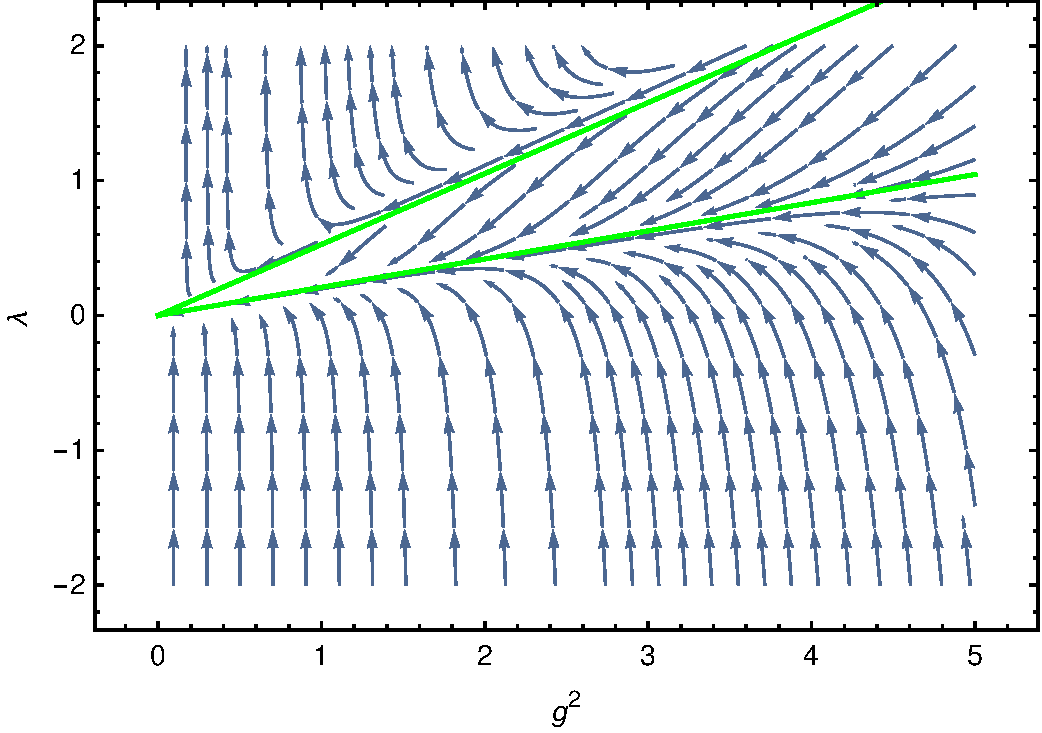
\includegraphics[width=9cm,clip]{pics/flow}
   \caption{Running of the squared gauge coupling $g^2$ and of the scalar quartic coupling $\lambda$ for a theory with SU(5) gauge group, $N_f=26$ fundamental fermions and $N_S =1$ fundamental scalars. The arrows indicate the direction of increasing energy. The green lines represent the fixed flow solutions of the renormalisation group equations, characterised by a constant ratio $\lambda/g^2$.}
  \label{flow_2D}
\end{figure}

\begin{table}[thb]
  \small
  \centering
  \caption{For different values of N, ranges in $N_f$ such that there exist completely asymptotically free solutions, in a theory with SU(N) gauge group, $N_f$ fundamental fermions and $N_S=1$ fundamental scalars.}
  \begin{tabular}{lll}\toprule
  $N$ & $N_f$  \\\midrule
  2 & No solutions \\
  3 & $15.93 < N_f < 16.25$ \\ 
  4 & 1$9.8 < N_f < 21.75$ \\
  5 & $23.56 < N_f < 27.25$ \\
  6 & $27.27 < N_f  < 32.75$ \\
  7 & $30.94 < N_f  < 38.25$ \\
  8 & $34.6 < N_f  < 43.75$ \\
  9 & $38.24 < N_f < 49.25$ \\
  10 & $41.88 < N_f < 54.75$ \\\bottomrule
  \end{tabular}
  \label{asympt_freedom}
\end{table}

\begin{figure}[thb] 
  \centering
  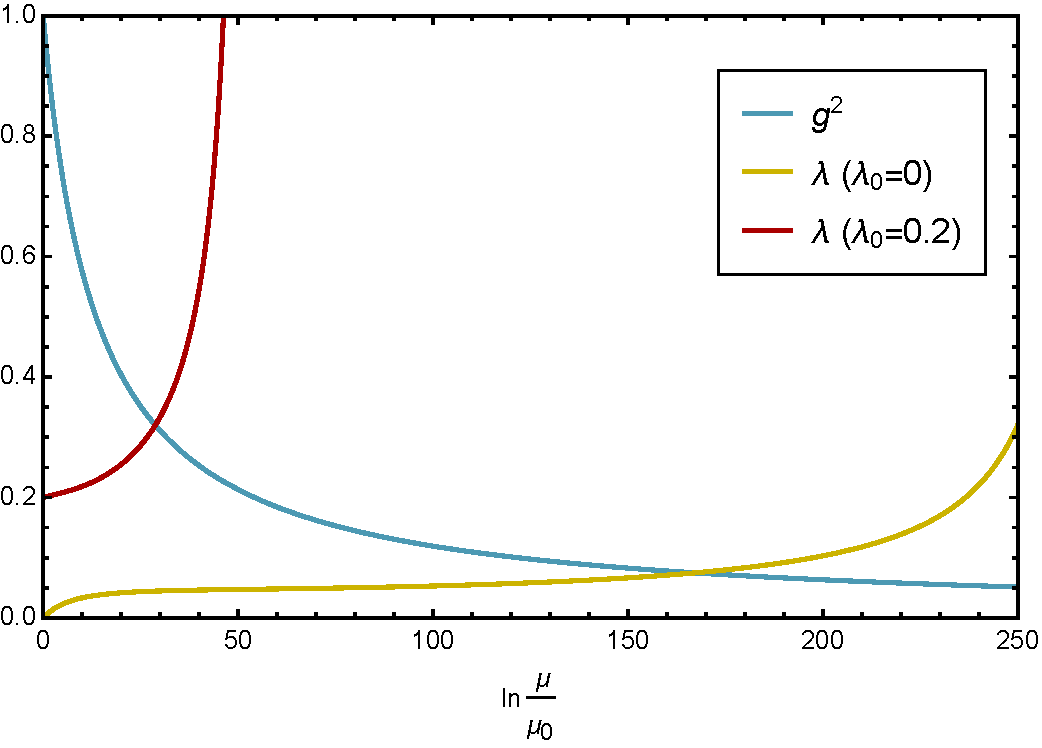
\includegraphics[width=9cm,clip]{pics/flow_N2}
  \caption{ Running of $g^2$ and $\lambda$ as functions of $\ln (\mu/\mu_0)$ in an SU(2) gauge theory with $N_f=2$ fundamental fermions and $N_S=1$ fundamental scalars. $\lambda$ is plotted for two different initial conditions: $\lambda_0 = \lambda(\mu_0) = 0$, and $\lambda_0=\lambda(\mu_0)=0.2$.}
  \label{flow_SU2}
\end{figure}

One more comment must be made regarding the case $N=2$. As previously pointed out, the fundamental representation of SU(2) is pseudo-real. One may wonder whether in this case there exist more quartic operators than the ones listed in equation \ref{quartic_operators}. It is shown in appendix \ref{app_quartic_potential} that, also in the case of an SU(2) gauge group, the most general quartic potential takes the form \ref{quartic_potential}.

%%%%%%%%%%%%%%%%%%%%%%%%%%%%%%%%%%%%%%%%%%%%%%%%%%%%%%

\section{Lattice setup}

%Motivations, what are we looking for on the lattice?
%verify symmetry breaking
%phase space of the lattice model
%spectrum
%Wilson coefficients?

\subsection{Action}

\subsection{Forces}
\label{Forces}

%%%%%%%%%%%%%%%%%%%%%%%%%%%%%%%%%%%%%%%%%%%%%%%%%%%%%%


\section{Spectrum}

\subsection{Mesons}

Finite volume corrections + dependence on $m_{PCAC}$

\subsection{Scalar states}

\subsection{Fermionic states}

%%%%%%%%%%%%%%%%%%%%%%%%%%%%%%%%%%%%%%%%%%%%%%%%%%%%%%


\section{Phase space}

\subsection{Phase diagram of the SU(2)-Higgs model}

\subsection{Gauge fixing}

\subsection{Results}

%%%%%%%%%%%%%%%%%%%%%%%%%%%%%%%%%%%%%%%%%%%%%%%%%%%%%%

\section{Conclusions and outlook}

%Renormalisation, continuum limit

%%%%%%%%%%%%%%%%%%%%%%%%%%%%%%%%%%%%%%%%%%%%%%%%%%%%%%
